%%%%%%%%%%%%%%%%%%%%%%% preamble %%%%%%%%%%%%%%%%%%%%%%%%%%%
\documentclass[10pt,letterpaper]{article}
\usepackage{opex3}
%\usepackage{graphicx}
\usepackage{hyperref}
\usepackage{amssymb}
\hypersetup{colorlinks=true,
		      urlcolor=blue}
\usepackage{amsmath}      
\usepackage{bm}
\newcommand{\myeqno}[1]{Eq.~\eqref{#1}}
\DeclareMathOperator*{\argmin}{arg\,min}
\DeclareMathOperator*{\argmax}{arg\,max}
%%%%%%%%%%%%%%%%%%%%%%% begin %%%%%%%%%%%%%%%%%%%%%%%%%%%%%%
%\linespread{1.25}
\begin{document}
\title{\Large{Problem set 1}}
\author{\href{mailto:rohan.kekatpure@gmail.com}{Rohan D. Kekatpure}}
\address{}
\email{}

%\begin{thebibliography}{9}
%\bibitem{mnist} 
%MNIST handwritten digit database.\\
%\href{\tt http://yann.lecun.com/exdb/mnist/}{http://yann.lecun.com/exdb/mnist/}
%
%\bibitem{ionosphere}
%Ionosphere data at UCI.\\
%\href{\tt https://archive.ics.uci.edu/ml/machine-learning-databases/ionosphere/ionosphere.names}{https://archive.ics.uci.edu/ml/machine-learning-databases/ionosphere/ionosphere.names}
%
%\bibitem{kegl}
%B.~Kegl and R.~Busa-Fekete
%{\it Boosting products of base classifiers} \\
%\href{\tt https://www.lri.fr/~kegl/research/PDFs/KeBu09.pdf}{https://www.lri.fr/~kegl/research/PDFs/KeBu09.pdf}
%\end{thebibliography}

\section{Problem 1}
\subsection{Derivation of error function}
Assume our training set is, 
\begin{equation}
	\{(x_1, y_1), (x_2, y_2), \ldots (x_n, y_n)\}
\end{equation}
where $y_i \in \{0, 1\}$. 

We want to learn a hypothesis $h$ that outputs the probability that $y_i = 1$ given the data point $x_i$. Explicitly, 
\begin{align}
  P(y_i = 1|h, x_i) &= h(x_i) \label{p1}\\
  P(y_i = 0|h, x_i) &= 1 - h(x_i) \label{p2}
\end{align}
Using a trick (Mitchell p. 169), these two equations can be combined as
\begin{equation}
	P(Y=y_i|h, x_i) = h(x_i)^{y_i}(1-h(x_i))^{1-y_i}
\end{equation}
When $y_i=1$ the second term drops out and and we get \eqref{p1}. When $y_i = 0$, the first term drops and we recover \eqref{p2}.

To derive the likelihood function, we have to assume that (1) all data points are independent and (2) the error terms are identically distributed (i.e. the probability distribution of the error terms does not depend on the input $x_i$). Under these assumptions, the likelihood function is:
\begin{equation}
  \label{lk1}
  P(D|h) = \prod_{i=1}^{n} h(x_i)^{y_i}(1-h(x_i))^{1-y_i}
\end{equation}

The maximum likelihood (ML) hypothesis is the one that maximizes \eqref{lk1}:

\begin{equation}
\label{hml}
 h_{ML} = \argmax_{h} \prod_{i=1}^{n} h(x_i)^{y_i}(1-h(x_i))^{1-y_i}
\end{equation}

Equivalently, we can simplify \eqref{hml} by taking natural logs of both sides. Also, since we're asked to derive the {\em error} function, we take the negative logarithm:
\begin{equation}
\label{eml}
\boxed{J_n = - \sum_{i=1}^{n} y_i \ln h(x_i) + (1-y_i) \ln(1-h(x_i))}
\end{equation}
\eqref{eml} is the error or cost function to minimize in case of non-deterministic functions. 

\subsection{Comparison to error function for deterministic function}
Below we compare the error terms obtained for deterministic and non-deterministic functions:
\begin{enumerate}
\item Both error functions are convex (sum of convex functions like `log' is convex), so both are equally amenable to be solved by standard optimization techniques.
\item For non-deterministic function, we had to assume that the individual error terms followed a Bernoulli distribution (i.e. a flip of a coin) instead of a Gaussian.
\item Because of unbounded functions like natural logs, the logistic error terms seems more susceptible to numerical instabilities due to noise in data (where the arguments of the log function get close to zero).
\end{enumerate}

\subsection{Neural network}
Non-deterministic functions cannot guaranteed to be linearly separable. So a neural network trained using the perceptron would not be able to find a decision boundary with certainty. A neural network trained using gradient descent would need to be used.

However, for gradient descent training, a neural network trained with least squares error function seeks maximum likelihood hypothesis under the assumption that training data is modeled by a Normally distributed noise added to the target function value. In contrast a neural network trained using cross entropy minimization will seek maximum likelihood hypothesis under the assumption that the observed boolean value is a probabilistic function of the input (Mitchell P. 171)

\subsection{Y continuous instead of discrete variable}
When $y$ is a probability (i.e., a continuous variable), then its a {\em regression} problem. The error function above \eqref{eml} does not make sense for a regression problem. In this case, it is preferable to perform an ordinary least-squares  (OLS) regression. 

\section{Problem 2}
\begin{figure}[!h]
  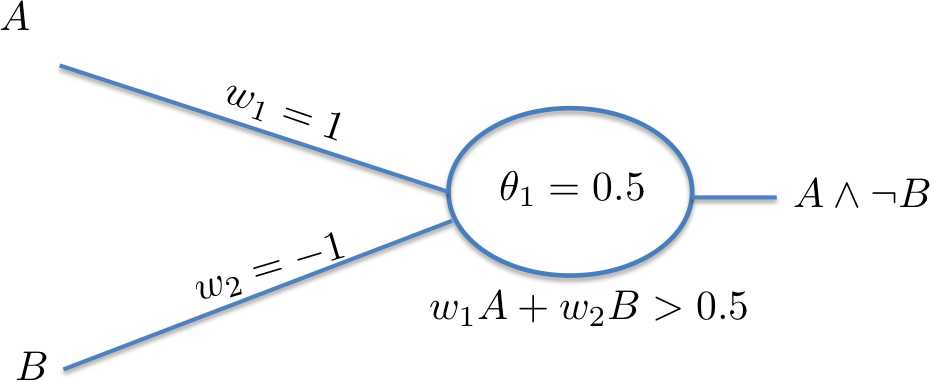
\includegraphics[width=2in]{./figures/anotb.png}
  \caption{Two input perceptron for $A\wedge\neg B$}
\end{figure}
%
\begin{figure}[!h]
  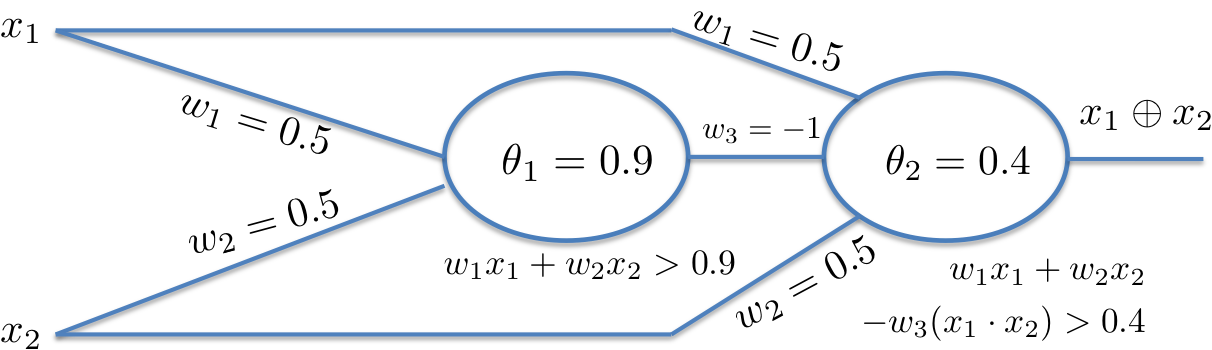
\includegraphics[width=3in]{./figures/xor.png}
  \caption{Two layer perceptron for $A\oplus B$}
\end{figure}

\section{Problem 3}
\subsection{Perceptron training}
The output of the perceptron now contains a quadratic term
\begin{equation}
  o = w_0 + w_1(x_1 +x_1^2) + w_2(x_2 + x_2^2) + \cdots + w_n(x_n + x_n^2)
\end{equation}
Perceptron training rule follows from Mitchell \S4.4.2 by replacing $x_i \to x_i + x_i^2$:
\begin{equation}
  \boxed{\Delta w_i = \eta (t - o) (x_i + x_i^2)}
\end{equation}
Note that $\Delta w_i > 0$ (i.e. weight should be increased) if $t > o$ and $x_i + x_i^2 > 0$ and vice versa.
\subsection{Gradient descent training}
For gradient descent, we use the component form of the training rule:
\begin{equation}
  \Delta w_i = -\eta \frac{\partial E}{\partial w_i}
\end{equation}
where $E$ is the sum-of-squared error function defined as 
\begin{equation}
  E(w) = \frac{1}{2} \sum_{d\in D}(t_d - o_d)^2
\end{equation}
Thus,
\begin{align}
  \frac{\partial E}{\partial w_i} &= \frac{1}{2} \frac{\partial}{\partial w_i} \sum_{d \in D}(t_i - o_i)^2 \nonumber \\
  &= \sum_{d \in D}(t_i - o_i) \frac{\partial}{\partial w_i} (t_i-o_i)\nonumber \\
  &= -\sum_{d \in D}(t_i - o_i) (x_{id}+x_{id}^2),
\end{align}
where $x_{id}$ refers to $i$'th component (feature) of the $d$'th training example. 

The GD training rule is thus:
\begin{equation}
  \boxed{  \Delta w_i = \eta\sum_{d \in D}(t_i - o_i) (x_{id}+x_{id}^2)}
\end{equation}

\section{Problem 4}

\begin{figure}[!h]
 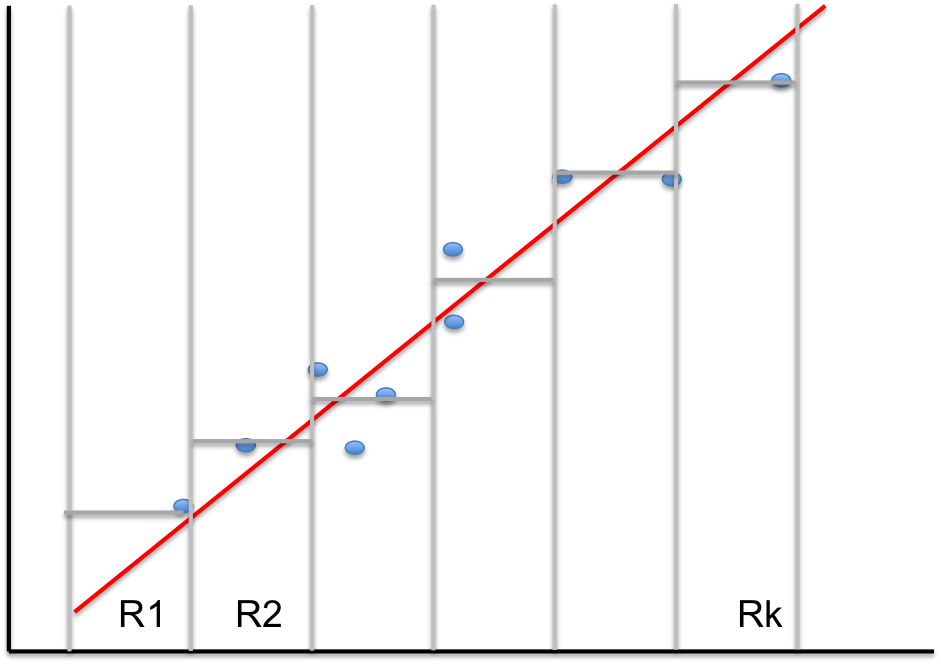
\includegraphics[width=3in]{./figures/regressiontrees.png}
 \caption{Regression trees\label{rtree}}
\end{figure}

{\bf Using decision trees for regression:} Decision trees can be used to perform regression by partitioning the feature space into suitable number of regions and assigning a target $y$ value to each region. A one-dimensional example is shown in figure \ref{rtree} where the X-axis is partitioned into segments and each segment is assigned a $y$ value shown by the horizontal line. 

The next question is the splitting criterion and choice of y-value. One possible choice, as mentioned in the problem statement, is a least squared error function. Under this choice, one can perform a recursive, greedy binary splits at every stage such that the sum of squares in each half plane is minimized. The procedure is then repeated recursively in every half plane until the stopping criterion (depth, number of leaves etc) is met. 

The $y$-value for each region $R_i$ is the {\em mean} of all $y$ values falling in that region. This statement can be proved in the following way. The total sum of squares is written in the usual way:
\begin{equation}{E = \sum_{i=1}^n (y_i - \hat{y}_i)^2}
\end{equation}
where $\hat{y}_i$ is the predicted output. According to our algorithm, $\hat{y}_i$ is a constant $y_r$ for region $R = r$. Thus the sum of squares can be written over each region $r$ as:
\begin{equation}
  E = \sum_{r\in R}\sum_{i=1}^{n_r} (y_i - y_r)^2
  \label{rss}
\end{equation}
where $n_r$ is the number of training examples with output falling in region $R = r$. We can find out all the $y_r$ values by minimizing \eqref{rss} with respect to $y_r$.
\begin{align}
  \frac{\partial E}{\partial y_r} &= 2\sum_{i=1}^{n_r}(y_i-y_r) \nonumber \\
  \frac{\partial E}{\partial y_r} = 0 & \Rightarrow \boxed{y_r = \frac{1}{n_r}\sum_{i=1}^{n_r}y_i}
\end{align}
In words, total sum of squares is minimized when the `constant' $y$-value in each leaf node is the average of the all $y$ values falling in that region. 

\subsection{Regression on Boston housing dataset:} Not implemented.
\section{Problem 6}

{\bf Short answer:} If the line defining the target function is known to be axis-parallel (i.e., parallel to one of the axes) then decision trees or KNN would perform equally well. If the line defining the target function is not axis parallel (i.e. at a non-zero angle to both axes), then I'd choose KNN. 

{\bf Rationale:} Decision trees splits divide the plane into axis-parallel rectangles. As such, when the data is not separable by axis parallel rectangles, decision trees tend to underperform. Particularly, decision trees face issues when classifying data points which are linearly separable but the separating line is {\em not} axis parallel. This leads to the `staircase' decision boundary. As such KNN seems to be a better choice since it does not suffer from the bias of choosing axis-parallel splits.

However, KNN could potentially suffer in the case when there is not enough training data.


\end{document}












